\section{Recursions}

\subsection{Definitions}

$S^1, S^2$ target and query sequences\\
$i_1, j_1, i_2, j_2$ interaction boundaries\\
$si_1, sj_1, si_2, sj_2$ seed boundaries\\
$N$ the maximum interaction length $(\sim 150)$\\
$M$ the enclosed unpaired positions in one loop $(\sim 15)$

General energy computation:

\begin{figure}[H]
	\centering
	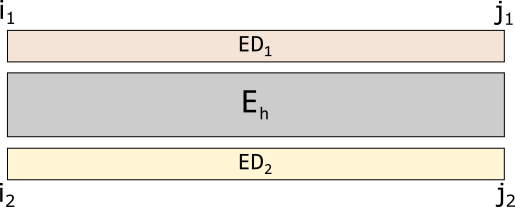
\includegraphics[scale=0.45]{seedenergy_general.png}
\end{figure}

\begin{equation*}
E(\substack{i_1,j_1\\i_2,j_2}) = E_{h}^{seed}(\substack{i_1,j_1\\i_2,j_2}) + ED_{1}(\substack{i_1\\j_1}) + ED_{2}(\substack{i_2\\j_2})
\end{equation*}

Optimization task:
\begin{equation*}
\min\limits_{seed}
\min\limits_{\substack{j_{1}-i_{1} \le N\\j_{2}-i_{2} \le N}}
\begin{pmatrix}
E_{h}^{seed}(\substack{i_1,j_1\\i_2,j_2})
\end{pmatrix}\\
\end{equation*}

\subsection{Initialization}

\begin{equation*}
\underset{{\substack{si_1 \le i_{1} \le j_{1} \le sj_{1}\\si_2 \le i_{2} \le j_{2} \le sj_{2}}}}{\forall} E_{h}^{seed}(\substack{i_1,j_1\\i_2,j_2}) = \infty
\end{equation*}

\begin{equation*}
E_{h}^{seed}(\substack{si_1,sj_1\\si_2,sj_2}) = E_{seed}
\end{equation*}

with $E_{seed}$ including $E_{init}$.

\clearpage

\subsection{Exact naive method ($O(N^{4})$ space + time)}

\begin{figure}[H]
	\centering
	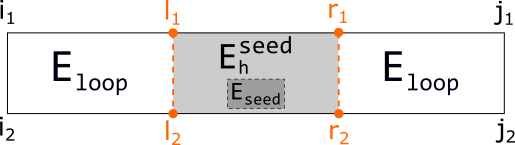
\includegraphics[scale=0.65]{seedenergy.png}
\end{figure}

\begin{equation*}
\substack{
  \underset{\substack{si_{1}-N \le i_{1} \le si_{1}\\si_{2}-N \le i_{2} \le si_{2}}}{\forall}\\
  \underset{\substack{sj_{1} \le j_{1} \le sj_{1}+N\\sj_{2} \le j_{2} \le sj_{2}+N}}{\forall}
}
E_{h}^{seed}(\substack{i_1,j_1\\i_2,j_2}) = \begin{cases}
  \infty\\
  \quad\text{: if } \text{ no matching base pair }\\
  \infty\\
  \quad\text{: if } j_{1} - i_{1} > N \text{ oder } j_{2} - i_{2} > N\\
  \min\limits_{\substack{i_{1} < l_{1} \le r_{1} < j_{1}\\i_{2} < l_{2} \le r_{2} < j_{2}\\l_{1} - i_{1} - 1 \le M\\j_{1}-r_{1}-1 \le M\\l_{2} - i_{2} - 1 \le M\\j_{2}-r_{2}-1 \le M}}
  \begin{pmatrix}
	E_{loop}(\substack{i_1,l_1\\i_2,l_2}) + E_{h}^{seed}(\substack{l_1,r_1\\l_2,r_2}) + E_{loop}(\substack{r_1,j_1\\r_2,j_2})
  \end{pmatrix}\\
  \quad\text{: otherwise.}\\
  
\end{cases}
\end{equation*}

\clearpage

\subsection{Exact memory efficient method ($O(N^{2})$ space + $O(N^{4})$ time)}

\begin{figure}[H]
	\centering
	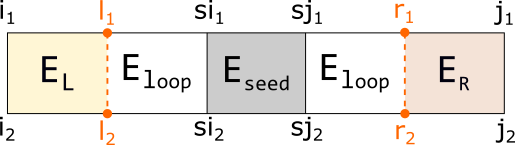
\includegraphics[scale=0.65]{seedenergy2.png}
\end{figure}

\begin{equation*}
E_{h}^{seed}(\substack{i_1,j_1\\i_2,j_2}) = \begin{cases}
\infty\\
\quad\text{: if } j_{1} - i_{1} > N \text{ oder } j_{2} - i_{2} > N\\
\begin{pmatrix}
E_{L}(\substack{i_1\\i_2}) + E_{seed} + E_{R}(\substack{j_1\\j_2})
\end{pmatrix}\\
\quad\text{: otherwise.}\\
\end{cases}
\end{equation*}

\begin{equation*}
\underset{\substack{si_{1}-N \le i_{1} \le si_{1}\\si_{2}-N \le i_{2} \le si_{2}}}{\forall}\\
E_L(\substack{i_1\\i_2}) = \begin{cases}
\infty\\
\quad\text{: if } \text{ no matching base pair }\\
\min\limits_{\substack{l_{1} - i_{1} - 1 \le M\\l_{2} - i_{2} - 1 \le M}}
\begin{pmatrix}
E_{loop}(\substack{i_1,l_1\\i_2,l_2}) + E_L(\substack{l_1\\l_2})
\end{pmatrix}\\
\quad\text{: otherwise.}\\

\end{cases}
\end{equation*}

\begin{equation*}
\underset{\substack{sj_{1} \le j_{1} \le sj_{1}+N\\sj_{2} \le j_{2} \le sj_{2}+N}}{\forall}
E_R(\substack{j_1\\j_2}) = \begin{cases}
\infty\\
\quad\text{: if } \text{ no matching base pair }\\
\min\limits_{\substack{j_{1}-r_{1}-1 \le M\\j_{2}-r_{2}-1 \le M}}
\begin{pmatrix}
E_R(\substack{r_1\\r_2}) + E_{loop}(\substack{r_1,j_1\\r_2,j_2})
\end{pmatrix}\\
\quad\text{: otherwise.}\\

\end{cases}
\end{equation*}

\clearpage

\subsubsection{Exact method (memory efficient) results}

Parameters:\\
master\_20: --qIntLenMax 20 --tIntLenMax 20 --threads 8\\
memory\_efficient\_20: --pred X -m M --qIntLenMax 20 --tIntLenMax 20 --threads 8\\
memory\_efficient\_ensemble\_20: --pred E -m M --qIntLenMax 20 --tIntLenMax 20 --threads 8\\

\begin{figure}[H]
	\centering
	\caption{Performance}
	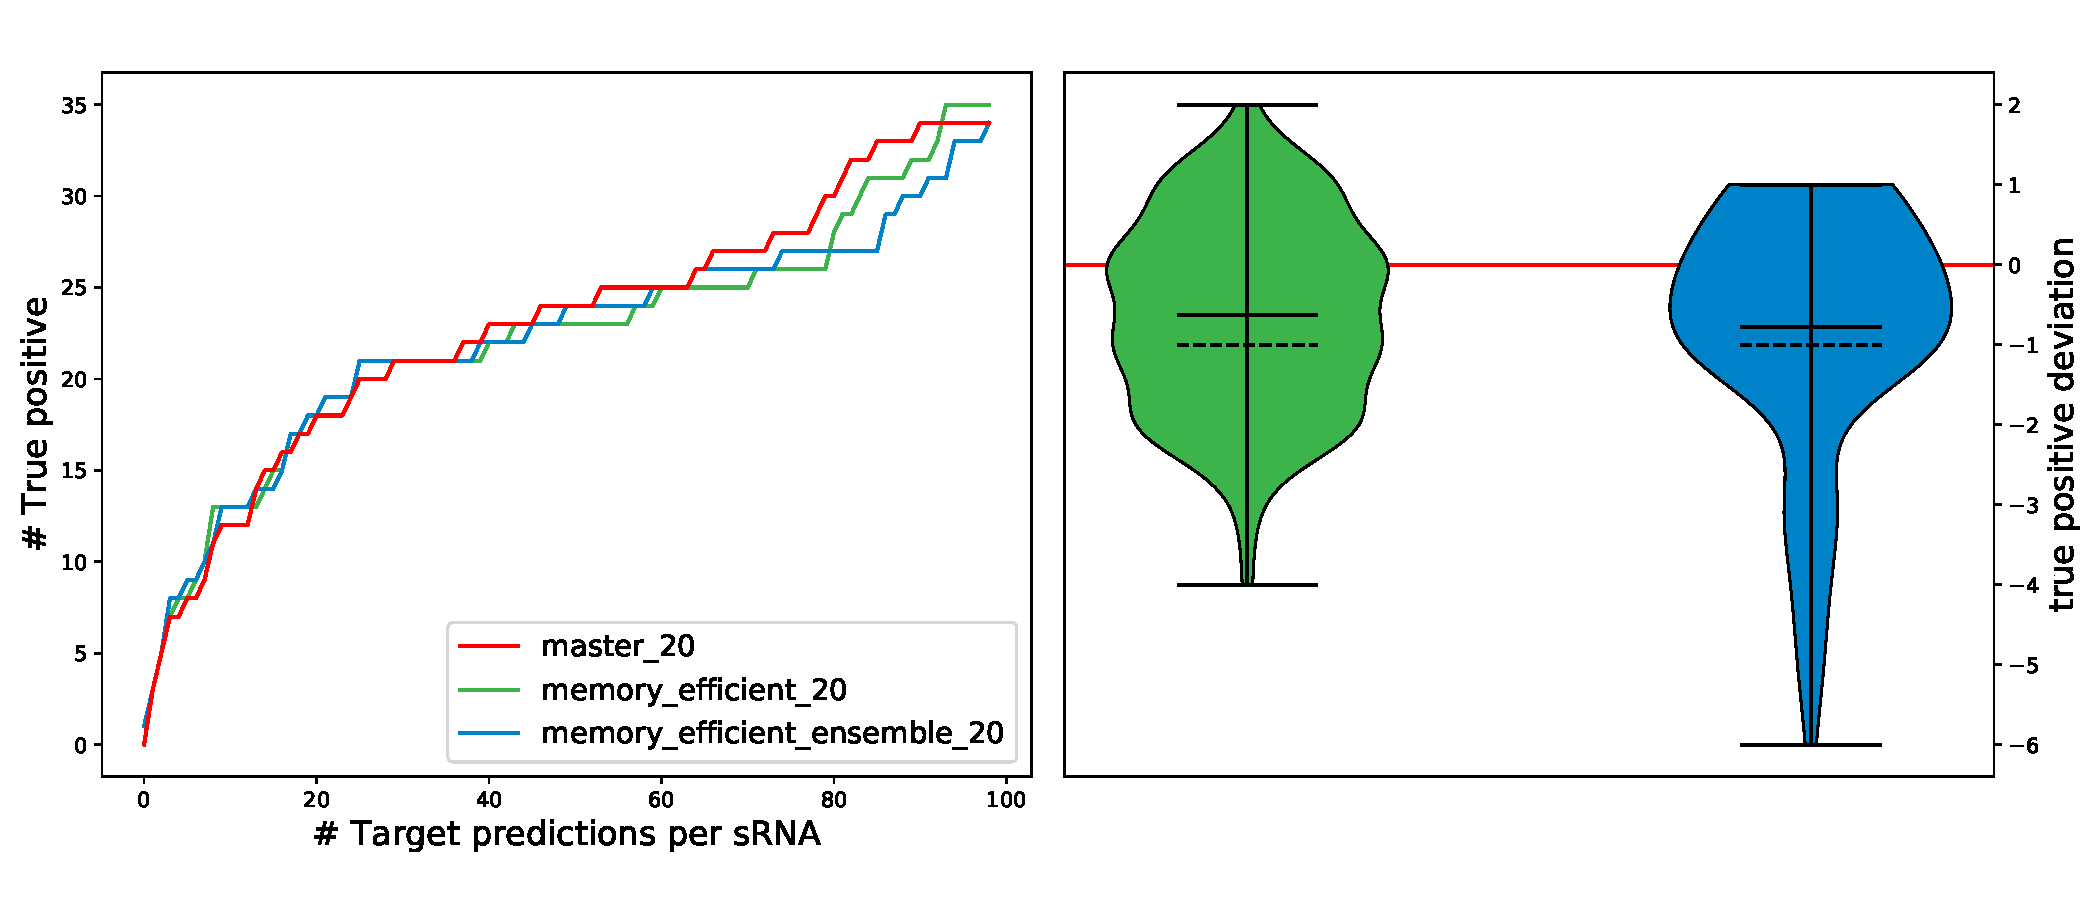
\includegraphics[scale=0.41]{memory_efficient_20.pdf}
\end{figure}

\begin{figure}[H]
	\centering
	\caption{Time \& memory}
	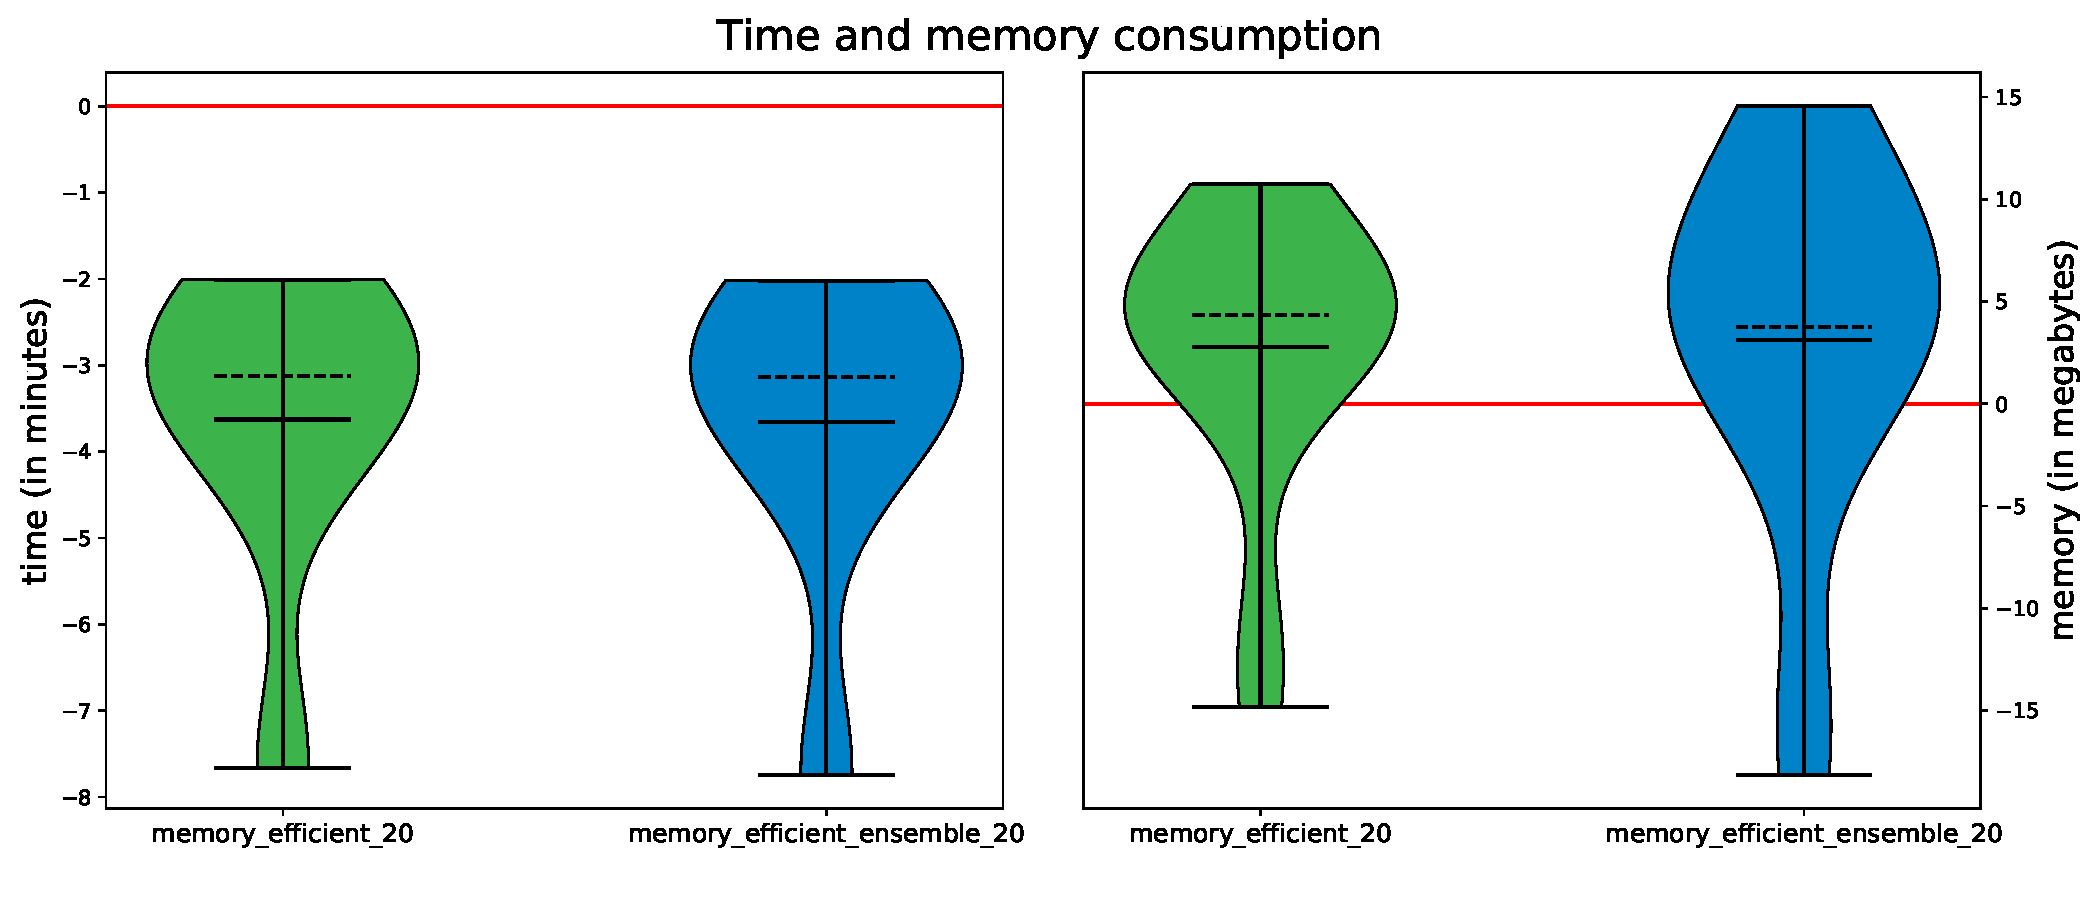
\includegraphics[scale=0.41]{memory_efficient_20_info.pdf}
\end{figure}

\clearpage

\subsection{Heuristic method ($O(N^{2})$ space + $O(N^{2})$ time)}

First find j1 and j2 that minimize right side. Call them $j_{1opt}$ and $j_{2opt}$. 

\begin{figure}[H]
	\centering
	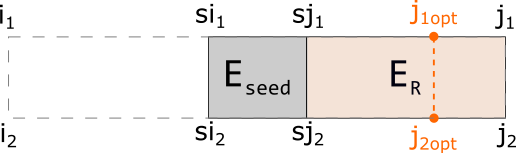
\includegraphics[scale=0.65]{seedenergy3.png}
\end{figure}

\begin{equation*}
\underset{j1, j2}{\arg\min}
\begin{pmatrix}
E_{seed} + E_{R}(\substack{sj_1,j_1\\sj_2,j_2})
\end{pmatrix}\\
\end{equation*}

with $E_{R}$ defined as in Recursion 2.\\
Then minimize over entire interaction up to $j_{1opt}$ and $j_{2opt}$.

\begin{figure}[H]
	\centering
	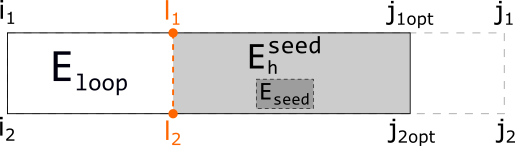
\includegraphics[scale=0.65]{seedenergy4.png}
\end{figure}

\begin{equation*}
\underset{\substack{si_{1}-N \le i_{1} \le j_{1}\\si_{2}-N \le i_{2} \le j_{2}}}{\forall}\\
E_{h}^{seed}(\substack{i_1, j_1\\i_2, j_2}) = \begin{cases}
\infty\\
\quad\text{: if } \text{ no matching base pair or $j_1 \neq j_{1opt}$ or $j_2 \neq j_{2opt}$ }\\
\min\limits_{\substack{l_{1} - i_{1} - 1 \le M\\l_{2} - i_{2} - 1 \le M}}
\begin{pmatrix}
E_{loop}(\substack{i_1,l_1\\i_2,l_2}) + E_{L}(\substack{l_1\\l_2}) + E_{seed} + E_{R}(\substack{j_{1opt}\\j_{2opt}})
\end{pmatrix}\\
\quad\text{: otherwise.}\\

\end{cases}
\end{equation*}

with $E_{L}$ and $E_{R}$ defined as in Recursion 2.\\

\clearpage

\subsubsection{Heuristic method results}

Parameters:\\
master\_20: --qIntLenMax 20 --tIntLenMax 20 --threads 8\\
heuristic\_20: --pred X -m H --qIntLenMax 20 --tIntLenMax 20 --threads 8\\
heuristic\_ensemble\_20: --pred E -m H --qIntLenMax 20 --tIntLenMax 20 --threads 8\\

\begin{figure}[H]
	\centering
	\caption{Performance}
	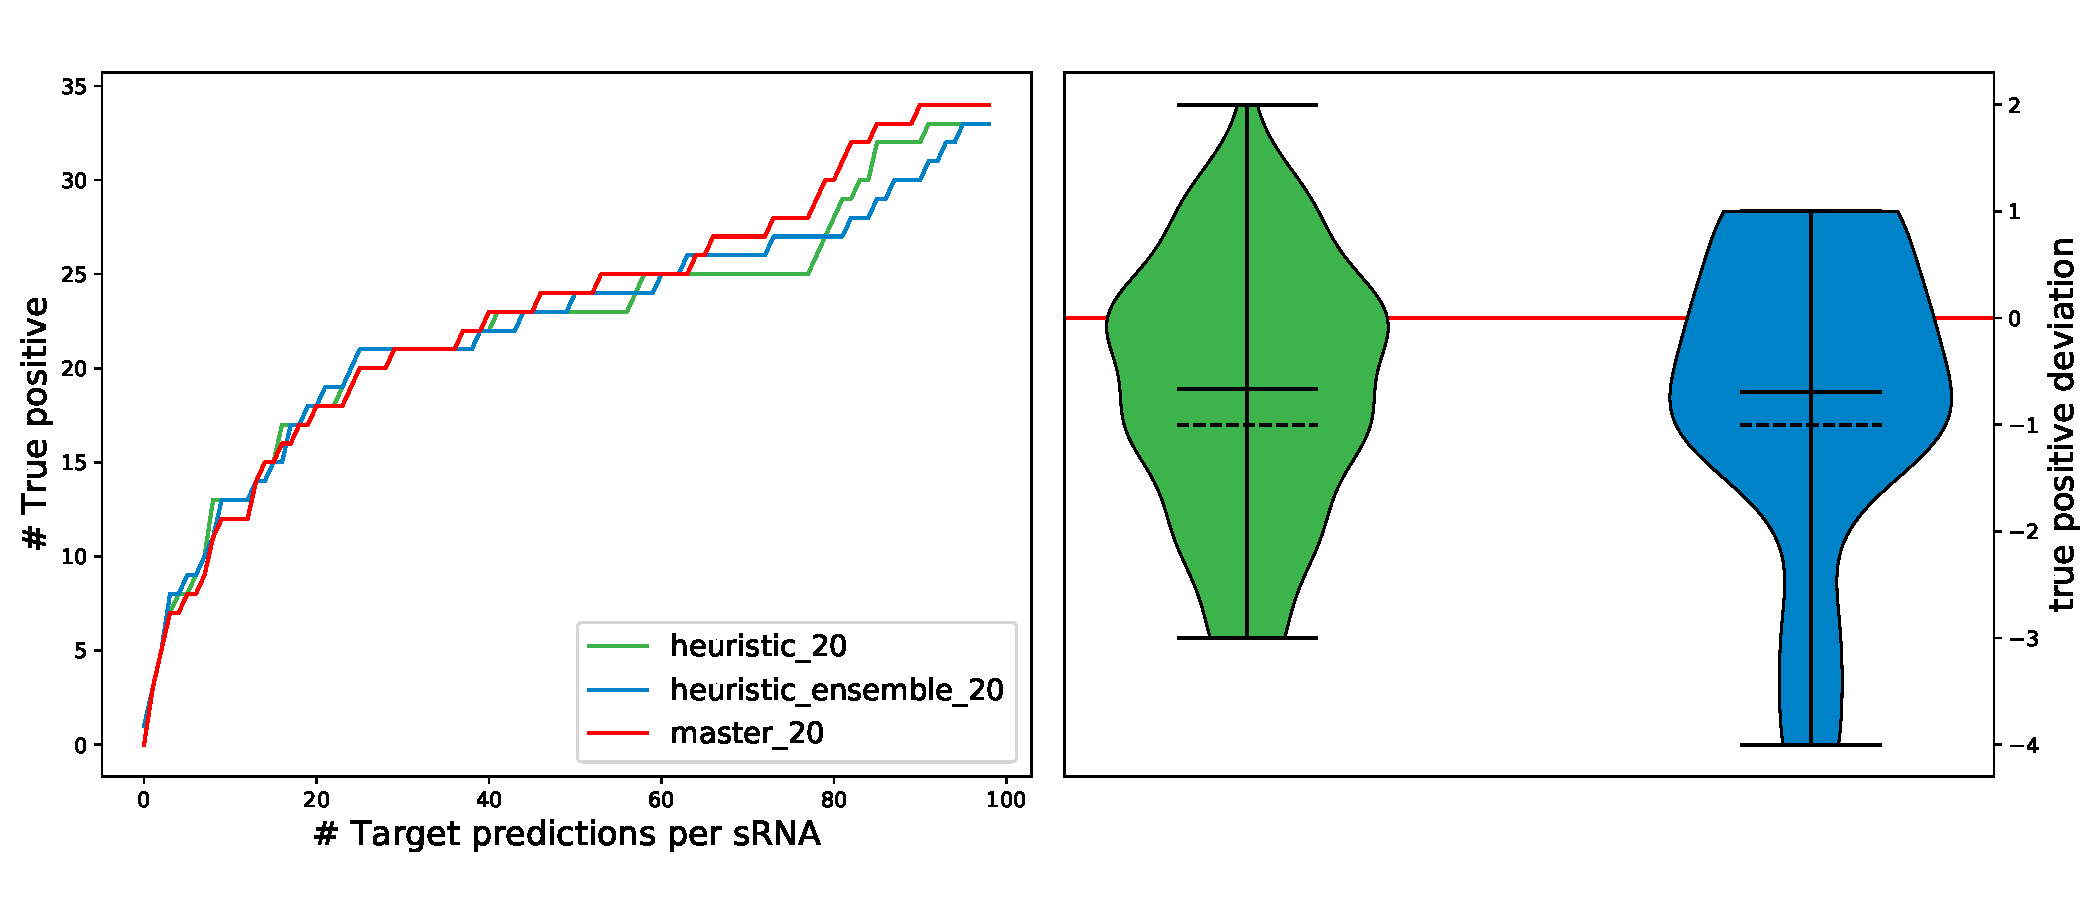
\includegraphics[scale=0.41]{heuristic_20.pdf}
\end{figure}

\begin{figure}[H]
	\centering
	\caption{Time \& memory}
	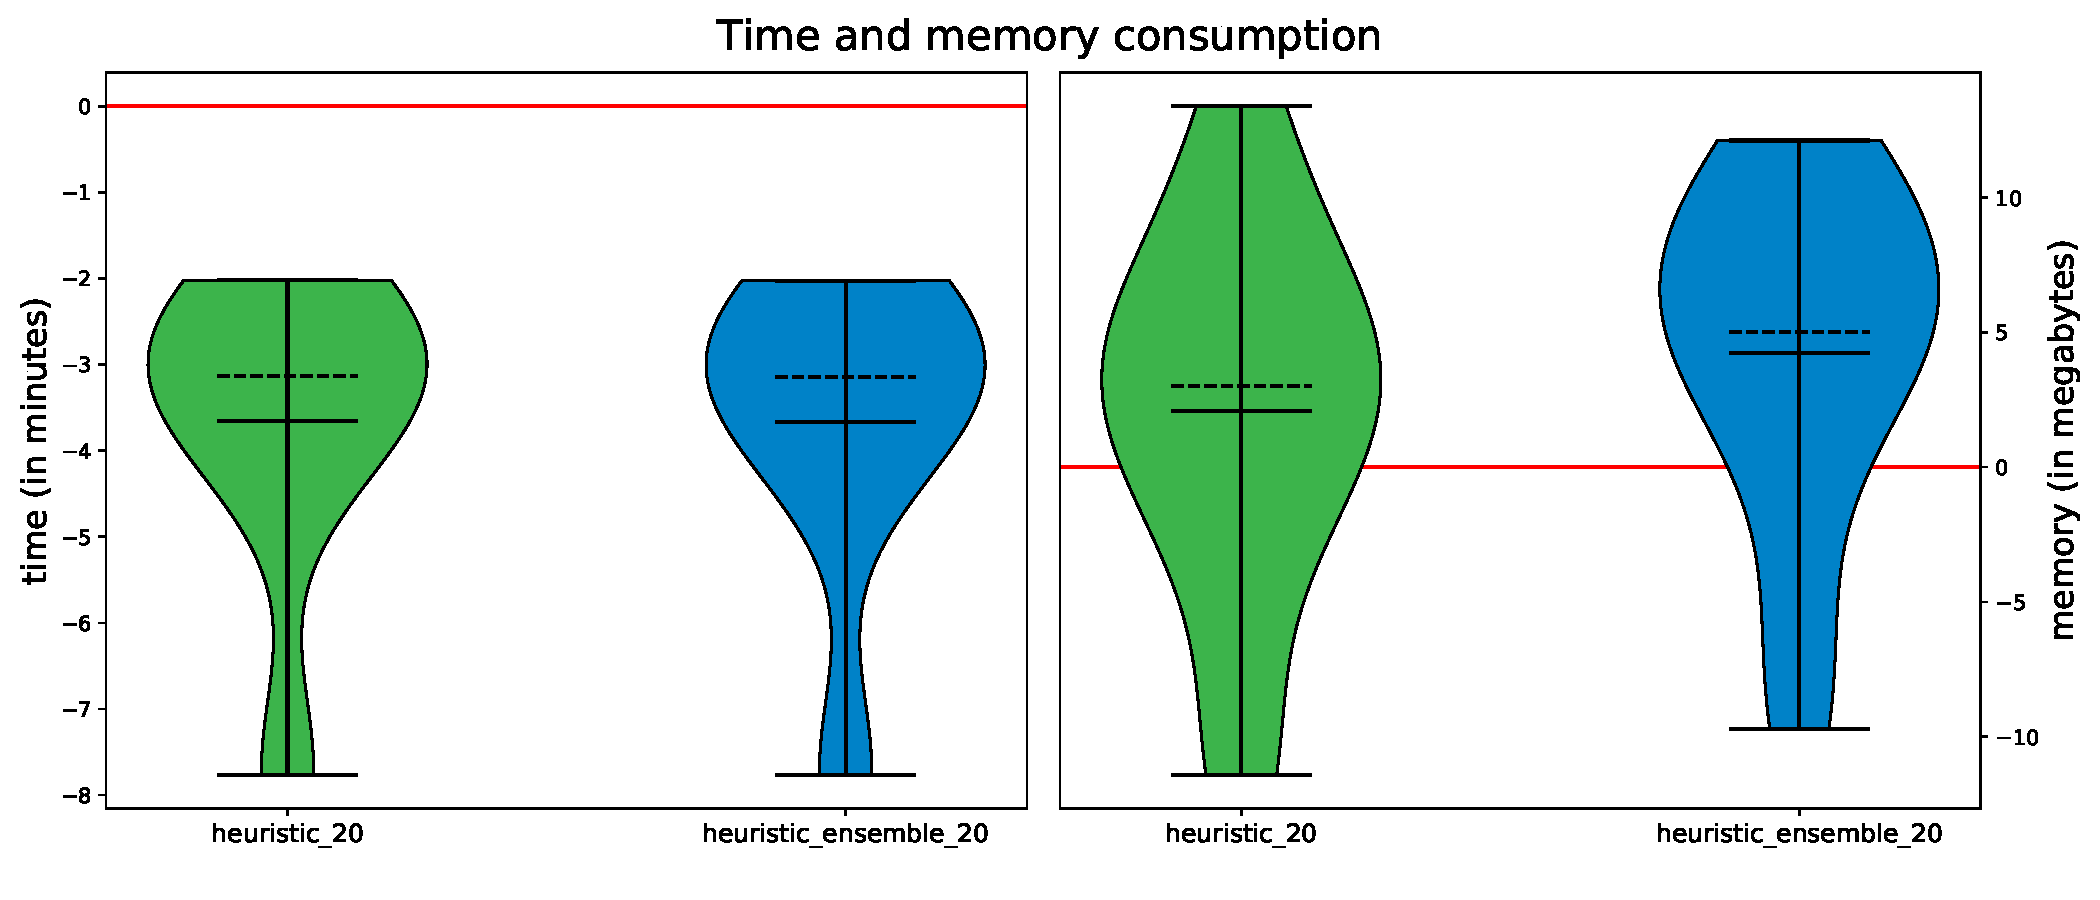
\includegraphics[scale=0.41]{heuristic_20_info.pdf}
\end{figure}

\clearpage

\subsection{RiBlast method}

* extend left + right without gaps\\
* extend left + right with gaps\\
* use approximated accessibility energies\\

\subsubsection{Parallel extension}

Given a seed, RiBlast first extends the interaction to the left and right of the seed without gaps. This means that we linearly loop over both sequences at the same time. If target and query nucleotides can pair, the new interaction energy is calculated. If it is lower than the present minimum, then the minimum is updated and the extension continues. If the minimum does not change for $drop\_out\_length\_wo\_gap$ steps, then the extension stops with $drop\_out\_length\_wo\_gap$ being an input parameter.
\\\\
Default $drop\_out\_length\_wo\_gap = 5$.

\begin{figure}[H]
	\centering
	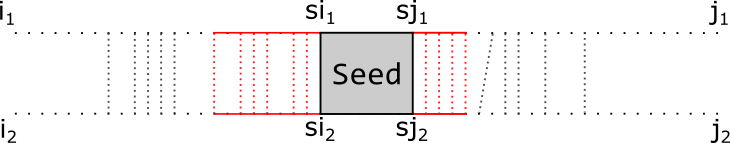
\includegraphics[scale=0.65]{riblast1.png}
\end{figure}

Example of gapless extension. The red lines indicate the range of extension. Here $drop\_out\_length\_wo\_gap$ is set to 2, meaning that the extension is stopped if the minimal energy does not improve after 2 steps.

\subsubsection{Thorough extension}

After the parallel extension finished, RiBlast does a second extension. This time gaps are allowed. This means that we loop over both sequences independently, resulting in a quadratic complexity. Again the minimum interaction energy is updated if a lower energy is found. If the minimum does not change for $drop\_out\_length\_w\_gap$ steps, then the extension stops with $drop\_out\_length\_w\_gap$ being an input parameter.
\\\\
Default $drop\_out\_length\_w\_gap = 16$.

\subsubsection{Accessibility energy}

\clearpage

\subsubsection{RiBlast method results}

Parameters:\\
master\_20: --qIntLenMax 20 --tIntLenMax 20 --threads 8\\
riblast\_20: --pred X -m R --qIntLenMax 20 --tIntLenMax 20 --threads 8\\

\begin{figure}[H]
	\centering
	\caption{Performance}
	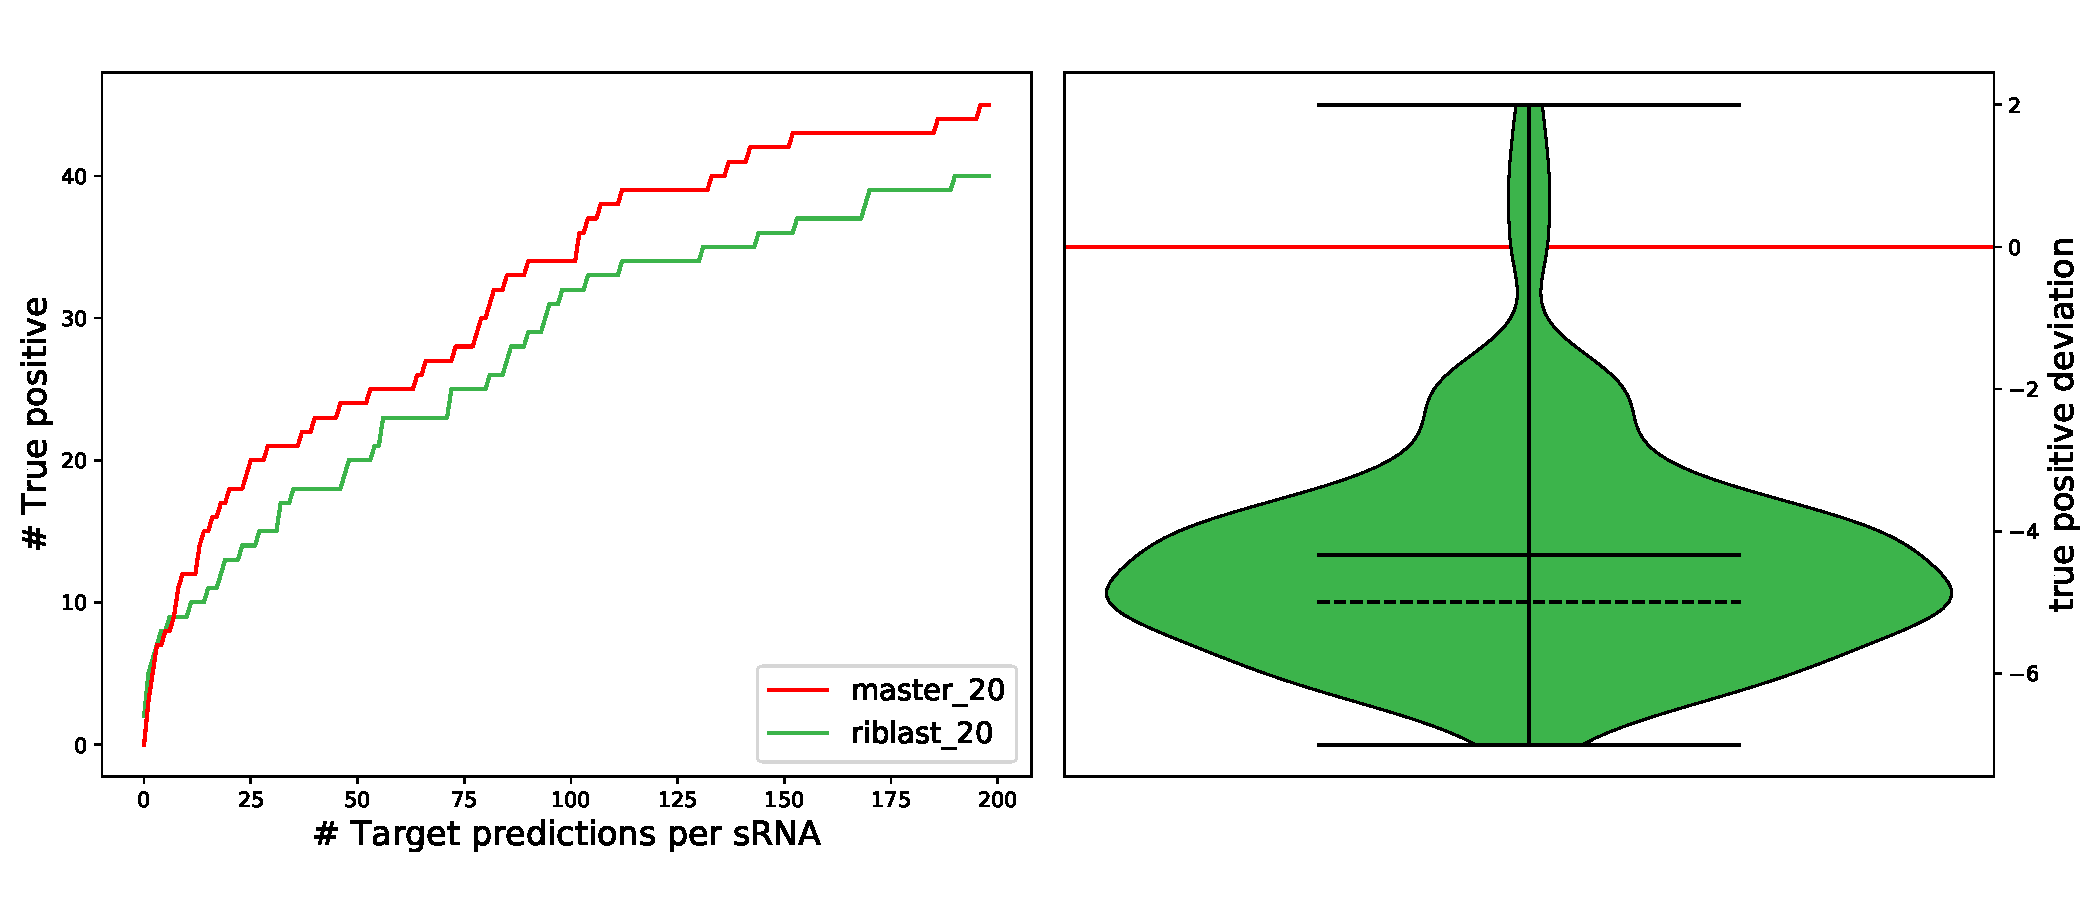
\includegraphics[scale=0.41]{riblast_20.pdf}
\end{figure}

\begin{figure}[H]
	\centering
	\caption{Time \& memory}
	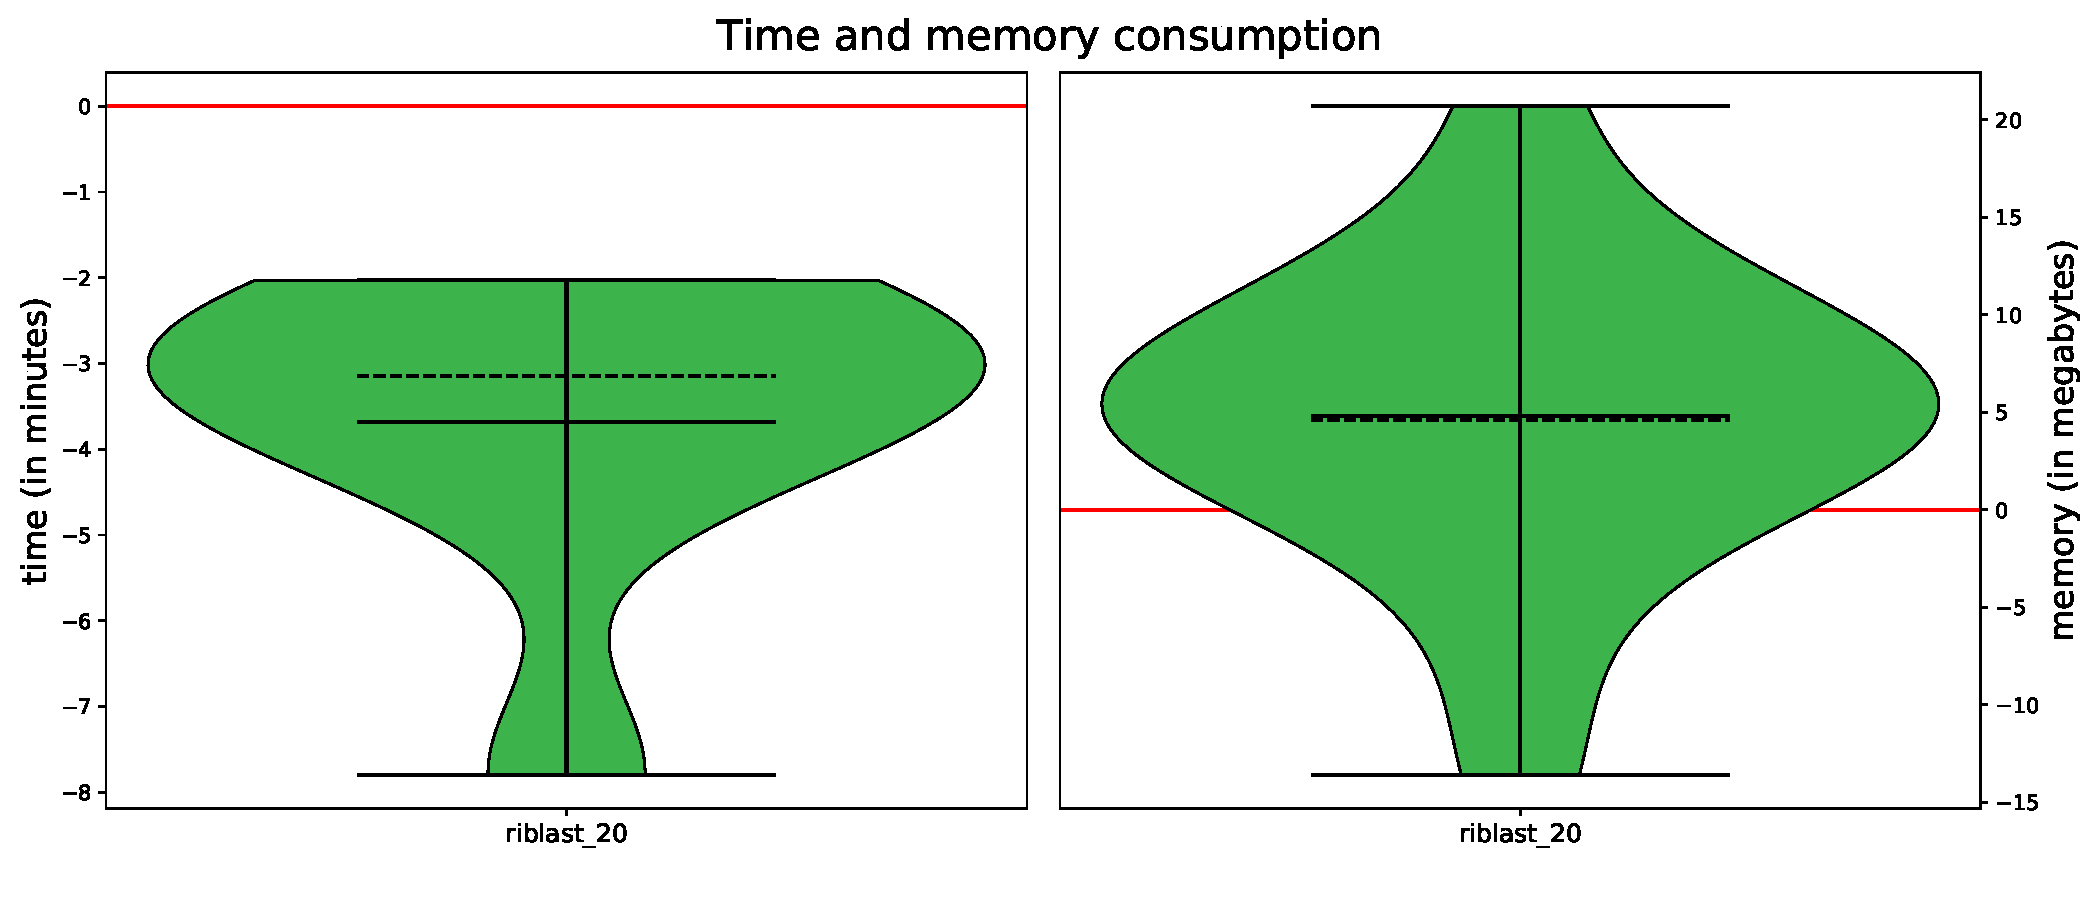
\includegraphics[scale=0.41]{riblast_20_info.pdf}
\end{figure}

RiBlast uses approximated accessibility energies as proposed in RNAplex-a.